% Version-specific figures. main.tex (v1) inputs figs_v1.tex; main_v2.tex inputs figs_v2.tex.
% The sections call \FigureEncSeeds (column width, in sec:encoder) and \FigureLLM (text width, in sec:llm).
% v1: the original figures (PNG renders from clarity/mideval_figures.py and clarity/e13_figures.py).

\newcommand{\FigureEncSeeds}{%
\begin{figure}[t]
\centering
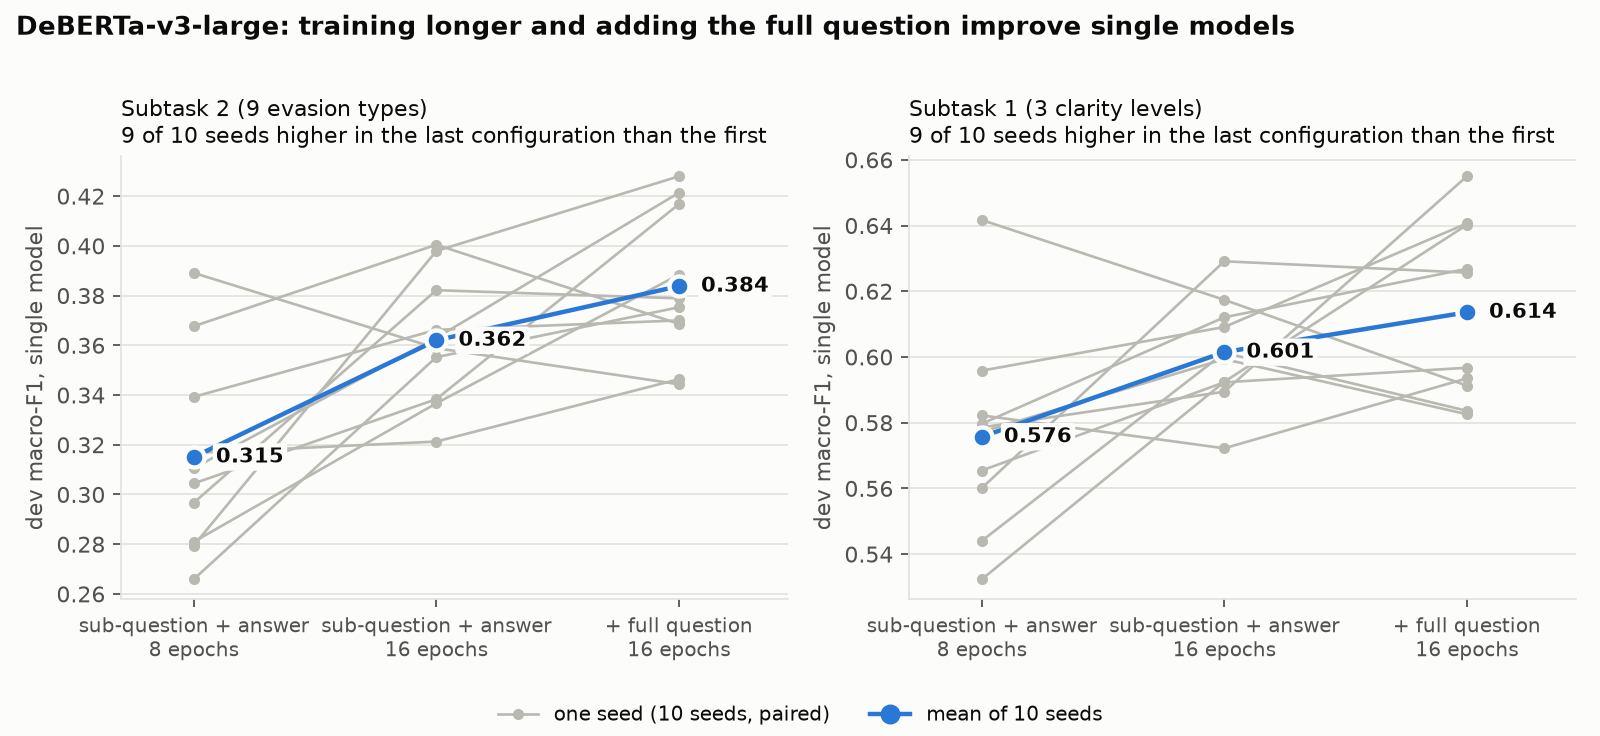
\includegraphics[width=\columnwidth]{figures/per_seed_progression.png}
\caption{Single DeBERTa-v3-large models on dev, per seed. Grey lines: one seed,
paired across the three configurations. Blue: mean of 10 seeds. Left: \Stwo; right:
\Sone.}
\label{fig:enc-seeds}
\end{figure}}

\newcommand{\FigureLLM}{%
\begin{figure*}[t]
\centering
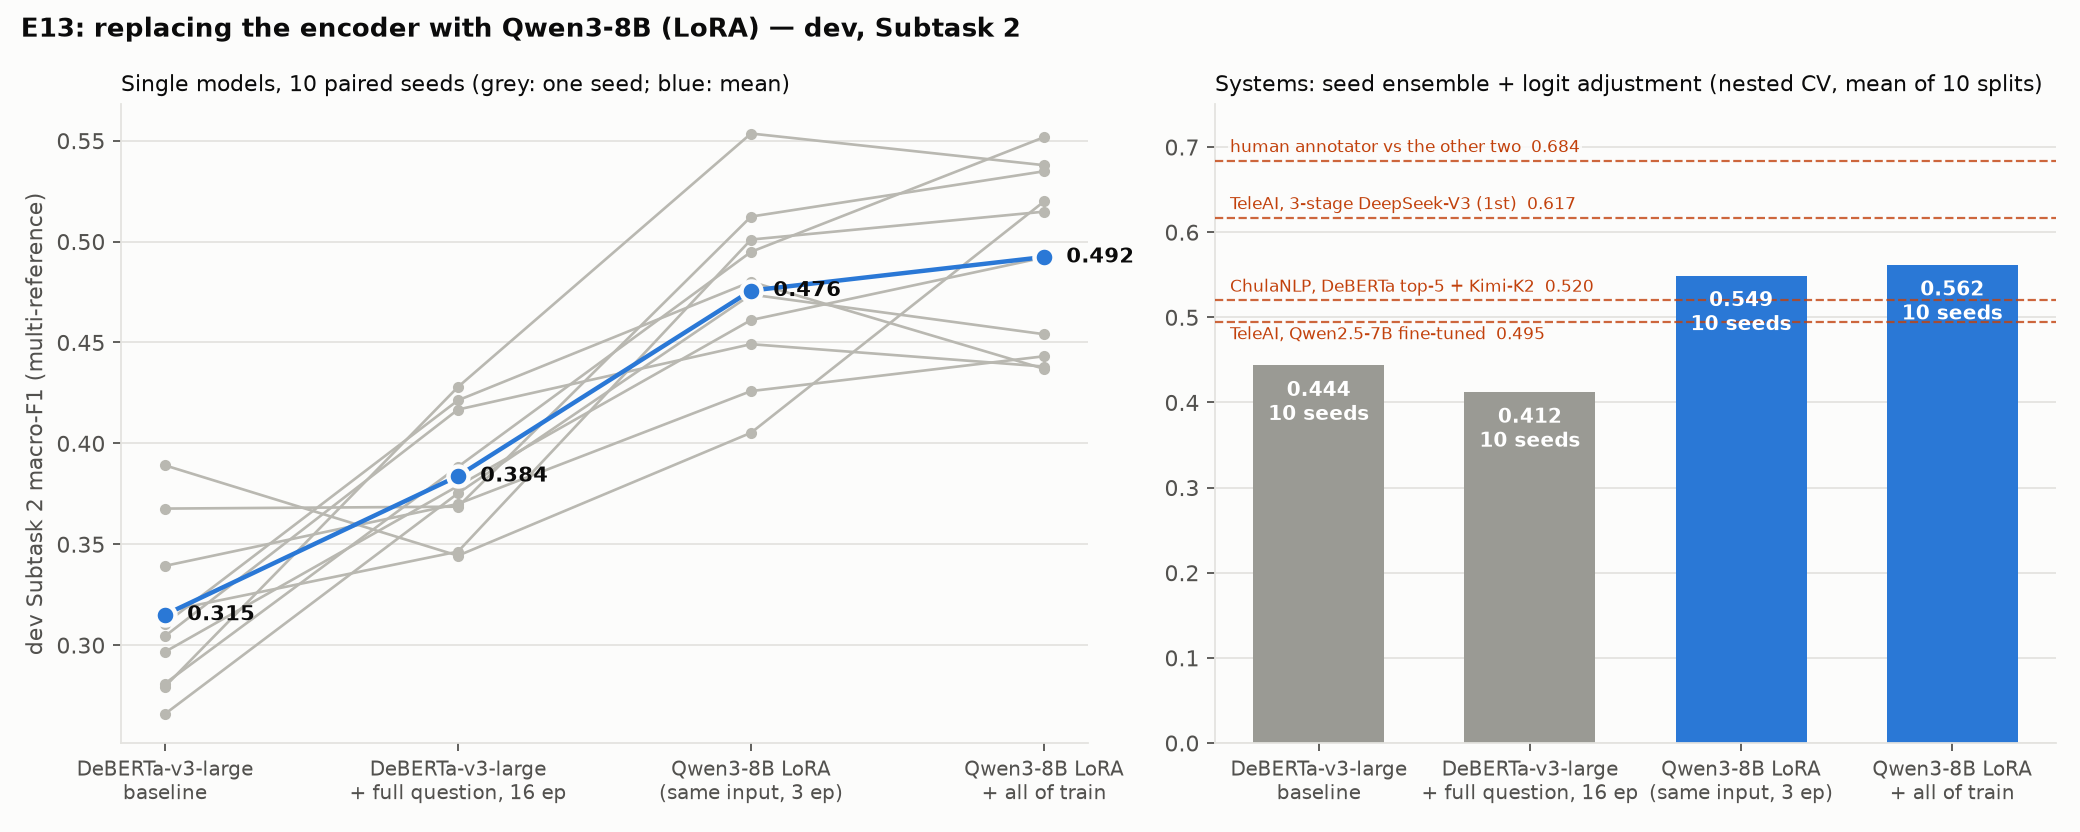
\includegraphics[width=\textwidth]{figures/e13_qwen_vs_deberta.png}
\caption{Dev \Stwo{} multi-reference macro-F1. \textbf{Left:} single models on 10 paired seeds (grey lines: one seed; blue: mean) for the DeBERTa-v3-large baseline, DeBERTa with the full question and 16 epochs, Qwen3-8B-Base with LoRA on the same input (3 epochs), and Qwen trained on all of train. \textbf{Right:} the corresponding 10-seed systems (ensemble + logit adjustment, nested CV; bars give the mean over 10 CV splits), with published dev references as dashed lines: TeleAI's multi-call pipeline (0.617) and fine-tuned Qwen2.5-7B (0.495) \citep{shi-etal-2026-teleai}, ChulaNLP's encoder+LLM pipeline (0.52) \citep{peerachaidecho-rutherford-2026-chulanlp}, and a human annotator scored against the other two (0.684).}
\label{fig:llm}
\end{figure*}}
